% Schematic of the gated HBV. Compile: pdflatex schematic_gated_hbv.tex, copy the PDF to figures/.
\documentclass[border=4pt]{standalone}
\usepackage[T1]{fontenc}
\usepackage{tikz}
\usetikzlibrary{arrows.meta, positioning, calc}
\definecolor{model}{HTML}{2E9E5B}
\definecolor{ink}{HTML}{222222}
\definecolor{storefill}{HTML}{DCF0E3}
\definecolor{grey}{HTML}{777777}
\begin{document}
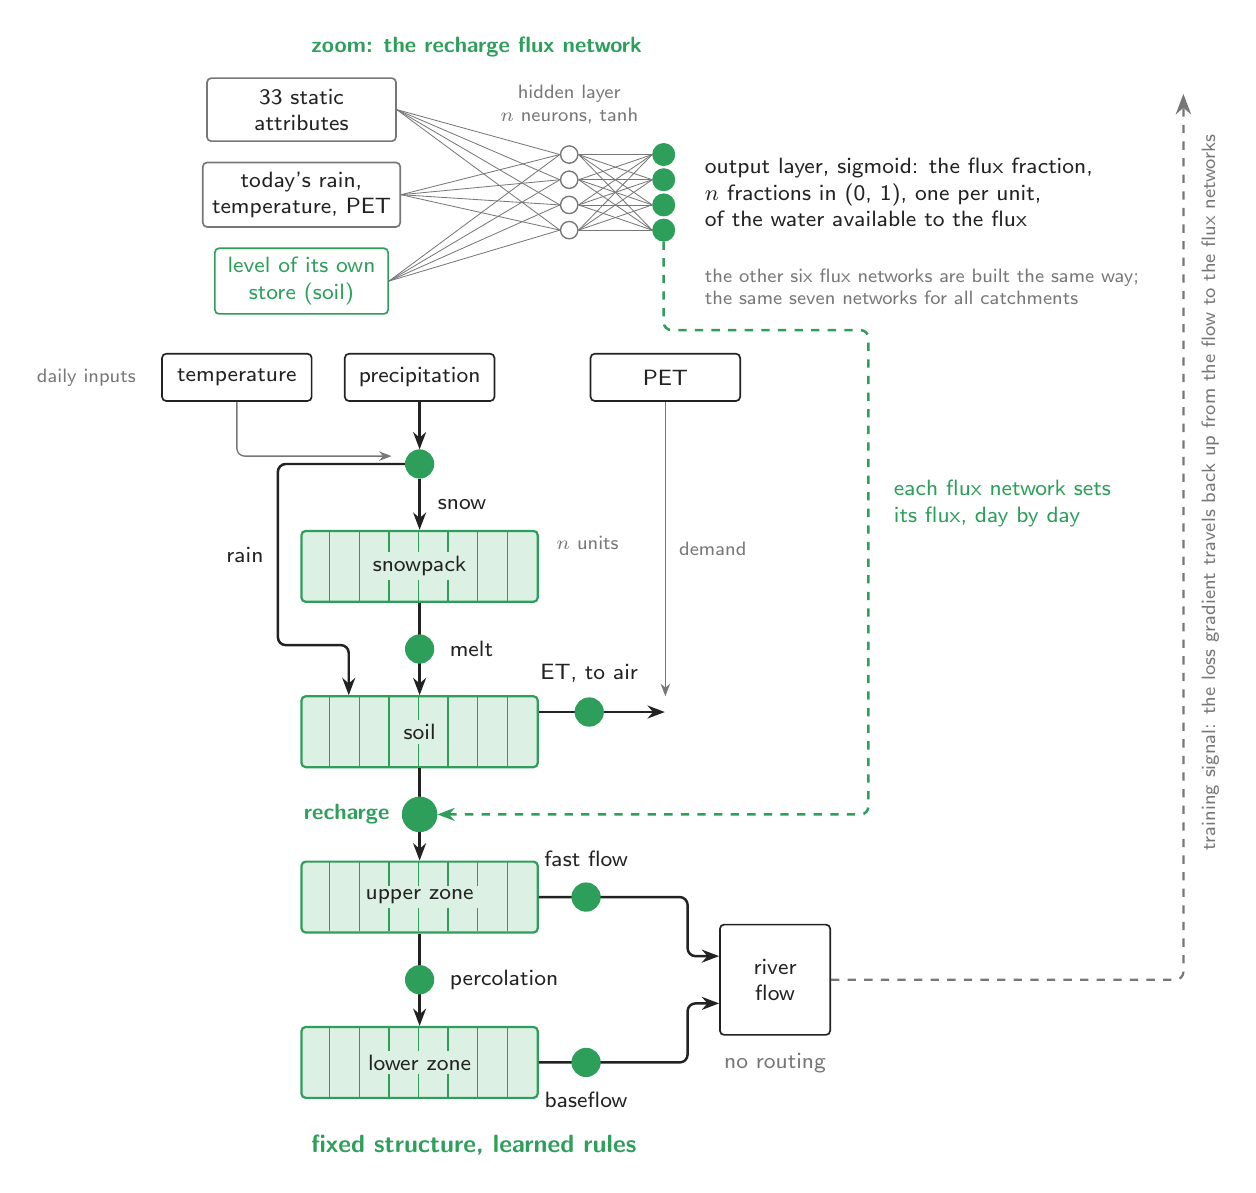
\begin{tikzpicture}[
  font=\sffamily\small, color=ink,
  store/.style={draw=model, fill=storefill, line width=0.8pt, minimum width=30mm, minimum height=9mm, rounded corners=1.5pt},
  flux/.style={-{Stealth[length=2.2mm]}, line width=0.9pt, color=ink, rounded corners=1mm},
  drives/.style={-{Stealth[length=1.6mm]}, line width=0.5pt, color=grey, rounded corners=1mm},
  lab/.style={font=\sffamily\footnotesize, color=ink, align=left},
  tie/.style={font=\sffamily\footnotesize, color=model, align=left},
  gate/.style={circle, draw=model, fill=model, line width=0.9pt, minimum size=3.4mm, inner sep=0pt},
  param/.style={-{Stealth[length=2.2mm]}, dashed, color=model, line width=0.9pt, rounded corners=1mm},
  grad/.style={-{Stealth[length=2.6mm]}, dashed, color=grey, line width=0.8pt, rounded corners=1mm},
  box/.style={draw=grey, line width=0.6pt, rounded corners=1.5pt, minimum height=8mm, align=center, font=\sffamily\footnotesize},
  input/.style={draw=ink, line width=0.6pt, rounded corners=1.5pt, minimum height=6mm, minimum width=19mm, align=center, font=\sffamily\footnotesize},
  neuron/.style={circle, draw=grey, fill=white, line width=0.5pt, minimum size=2.2mm, inner sep=0pt},
]
% ---- what every gate reads -> a small network per gate -> a fraction
\node[box, minimum width=24mm] (att) at (0, 0) {33 static\\attributes};
\node[box, minimum width=22mm, below=2.5mm of att] (tod) {today's rain,\\temperature, PET};
\node[box, minimum width=22mm, below=2.5mm of tod, draw=model, color=model] (own) {level of its own\\store (soil)};
\foreach \i in {1,...,4}  {\node[neuron] (h\i) at (34mm, {(2.5-\i)*3.2mm - 10.5mm}) {};}
\foreach \i in {1,...,4} {\node[gate, minimum size=2.6mm] (o\i) at (46mm, {(2.5-\i)*3.2mm - 10.5mm}) {};}
\coordinate (g0) at (46mm, -10.5mm);
\foreach \b in {att, tod, own} {\foreach \j in {1,...,4} {\draw[grey, line width=0.3pt] (\b.east) -- (h\j.west);}}
\foreach \i in {1,...,4} {\foreach \j in {1,...,4} {\draw[grey, line width=0.3pt] (h\i.east) -- (o\j.west);}}
\node[lab, color=grey, font=\sffamily\scriptsize, align=center, anchor=south] at (34mm, -3mm) {hidden layer\\$n$ neurons, tanh};
\node[lab, anchor=west, align=left] at (50mm, -10.5mm) {output layer, sigmoid: the flux fraction,\\$n$ fractions in (0, 1), one per unit,\\of the water available to the flux};
\node[lab, color=model, font=\sffamily\footnotesize\bfseries, anchor=south west] at (0mm, 5.5mm) {zoom: the recharge flux network};
\node[lab, color=grey, font=\sffamily\scriptsize, align=left, anchor=north west] at (50mm, -19mm) {the other six flux networks are built the same way;\\the same seven networks for all catchments};

% ---- the daily inputs, one row
\node[input] (pin) at (15mm, -34mm) {precipitation};
\node[input, left=4mm of pin] (tin) {temperature};
\node[input, right=12mm of pin] (petin) {PET};
\node[lab, color=grey, font=\sffamily\scriptsize, left=2mm of tin] {daily inputs};

% ---- the store chain, each store as n units
\node[gate] (gs) at (15mm, -45mm) {};
\node[store] (sp) at (15mm, -58mm) {};
\node[store] (sm) at (15mm, -79mm) {};
\node[store] (suz) at (15mm, -100mm) {};
\node[store] (slz) at (15mm, -121mm) {};
\foreach \s/\t in {sp/snowpack, sm/soil, suz/upper zone, slz/lower zone} {
  \foreach \i in {1,...,7} {\draw[model, line width=0.4pt] ($(\s.north west)+(\i*30mm/8,0)$) -- ++(0,-9mm);}
  \node[lab, fill=storefill, inner sep=1.5pt] at (\s) {\t};
}
\node[lab, color=grey, font=\sffamily\scriptsize, anchor=west] at ($(sp.east)+(1mm,3mm)$) {$n$ units};
\draw[flux] (pin) -- (gs);
\draw[flux] (gs) -- (sp) node[midway, right=1mm, lab] {snow};
\draw[flux] (gs.west) -| (-3mm, -68mm) node[pos=0.75, left=0.5mm, lab] {rain} -| ($(sm.north)+(-9mm,0)$);
\draw[flux] (sp) -- (sm) node[midway, gate] {} node[midway, right=2.5mm, lab] {melt};
\draw[flux] ($(sm.east)+(0,2.5mm)$) -- ++(16mm,0) node[pos=0.4, gate] {} node[pos=0.4, above=2.5mm, lab] {ET, to air};
\draw[flux] (sm) -- (suz) node[midway, gate, minimum size=4.2mm] (rg) {} node[midway, left=2.5mm, lab, color=model, font=\sffamily\footnotesize\bfseries] {recharge};
\draw[flux] (suz) -- (slz) node[midway, gate] {} node[midway, right=2.5mm, lab] {percolation};
% what drives the snow gate and ET (thin grey)
\draw[drives] (tin.south) |- ($(gs.west)+(-3mm,1mm)$) -- ($(gs.west)+(-1.7mm,1mm)$);
\draw[drives] (petin.south) -- ($(petin.south |- sm.east)+(0,4.5mm)$) node[pos=0.5, right=0.5mm, lab, color=grey, font=\sffamily\scriptsize] {demand};
% river
\node[box, draw=ink, minimum width=14mm, minimum height=14mm] (q) at ($(suz.east)!0.5!(slz.east)+(30mm,0)$) {river\\flow};
\draw[flux] (suz.east) -- ++(12mm,0) node[pos=0.5, gate] {} node[pos=0.5, above=2.5mm, lab] {fast flow} -| ($(q.west)+(-4mm,3mm)$) -- ($(q.west)+(0,3mm)$);
\draw[flux] (slz.east) -- ++(12mm,0) node[pos=0.5, gate] {} node[pos=0.5, below=2.5mm, lab] {baseflow} -| ($(q.west)+(-4mm,-3mm)$) -- ($(q.west)+(0,-3mm)$);
\node[lab, below=1mm of q, color=grey, align=center] {no routing};

% ---- the gates set the fluxes: one arrow into the middle of the chain
\draw[param] (o4.south) -- (46mm, -28mm) -| (72mm, -89.5mm) -- (rg.east);
\node[tie, anchor=west] at (74mm, -50mm) {each flux network sets\\its flux, day by day};



\coordinate (gx) at (112mm, 0);
\draw[grad] (q.east) -- (q.east -| gx) -- (112mm, 2mm) node[pos=0.55, anchor=north, xshift=1mm, lab, color=grey, font=\sffamily\scriptsize, rotate=90] {training signal: the loss gradient travels back up from the flow to the flux networks};
% ---- footer
\node[lab, color=model, font=\sffamily\small\bfseries, anchor=north west] at (0mm, -129mm) {fixed structure, learned rules};
\end{tikzpicture}
\end{document}
